\section{连续信号}

本节介绍连续信号,并给出4种基本的连续信号。

本节要点:
\begin{itemize}
    \item 掌握连续信号的概念;
    \item 熟悉4个基本连续信号。
\end{itemize}

%============================================================
\subsection{连续信号的概念}

\begin{definition}[连续信号]
当时间变量$t$取值实数时,我们称信号为{\bf 连续信号}(continuous-time signal)或{\bf 模拟信号}(analog signal),通常记为$x\left( t \right) $。
\end{definition}

%============================================================
\subsection{正弦信号}

\[
x\left( t \right) =A\sin \left( \omega t+\varphi \right)
\]
\begin{itemize}
    \item $A$:振幅;
    \item $\omega $:角频;
    \item $\varphi $:相位。
\end{itemize}
周期和频率:
\[
T=\frac{2\pi}{\omega} \qquad f=\frac{1}{T}=\frac{\omega}{2\pi} \qquad \omega =2\pi f
\]

%============================================================
\subsection{指数信号}

\[
x\left( t \right) =Ae^{at}
\]

当$a$为实数,信号的定义域和值域都是实数,称为{\bf 实指数信号}。
当$a>0$时,信号发散,如原子弹爆炸;当$a<0$时,信号衰减;当$a=0$时,信号为常数。
在实际系统中,一般信号都是衰减信号,所以写成:
\[
x\left( t \right) =Ae^{-\frac{t}{\tau}} \qquad \tau >0,t\geqslant 0
\]
其中,$\tau $称为{\bf 时间常数},反映了信号的衰减速度。

\begin{tcolorbox}
曲线$x\left( t \right) =Ae^{-\frac{t}{\tau}}$过曲线上点$\left( t_0,Ae^{-\frac{t_0}{\tau}} \right) $的切线方程:
\[
x\left( t \right) -Ae^{-\frac{t_0}{\tau}}=-\frac{A}{\tau}e^{-\frac{t_0}{\tau}}\left( t-t_0 \right)
\]
交于{\it t}轴:
\begin{align*}
&\because -Ae^{-\frac{t_0}{\tau}}=-\frac{A}{\tau}e^{-\frac{t_0}{\tau}}\left( t-t_0 \right) \\
&\therefore t=t_0+\tau
\end{align*}
这里可以得到衰减的实指数信号的一个特征,曲线切线与{\it t}轴的交点和切点的时间差永远是$\tau $。
\end{tcolorbox}

当$a$为复数$s=\sigma +i\omega $时信号为:
\[
x\left( t \right) =Ae^{st}
\]
此时信号的值域都是复数,称为{\bf 复指数信号},模、实部和虚部如下:
\begin{align*}
&\left| x\left( t \right) \right|=Ae^{\sigma t} \\
&\mathrm{Re}\left[ x\left( t \right) \right] =Ae^{\sigma t}\mathrm{Re}\left[ e^{i\omega t} \right] =Ae^{\sigma t}\cdot \cos \left( \omega t \right) \\
&\mathrm{Im}\left[ x\left( t \right) \right] =Ae^{\sigma t}\mathrm{Im}\left[ e^{i\omega t} \right] =Ae^{\sigma t}\cdot \sin \left( \omega t \right)
\end{align*}
实部和虚部都是正弦信号,且$T=2\pi /\omega $,两者“对称”振荡,整体由指数包络。
$\sigma $决定发散还是衰减,系统能量:
\[
E_{\infty}=\int_0^{+\infty}{\left| Ae^{st} \right|^2dt}=A^2\int_0^{+\infty}{e^{2\sigma t}dt}=\frac{A^2}{2\sigma}\left( \left. e^{2\sigma t} \right|_{0}^{+\infty} \right)
\]
当时$\sigma <0$,信号是有限能量。

物理中,复指数较实指数更为普遍。复指数代表着两个状态或者两种能量的相互转化,如弹簧的简谐振动、RC振荡电路。
$\omega $决定了转化速度,$\sigma $决定了系统是否对外辐射能量。
所以在复指数中,一个变量$s=\sigma +i\omega $就表示了系统的内在运动和对外关系。

当$s$为纯虚数时,写为:
\[
x\left( t \right) =Ae^{i\omega t}=A\left( \cos \omega t+i\sin \omega t \right)
\]
称为{\bf 纯虚指数信号}。
只有当$s$为纯虚数时,信号才是周期信号。
纯虚指数信号另一个特征是有限功率:
\[
P_{\infty}=\underset{T\rightarrow \infty}\lim \frac{1}{T}\int_{-\frac{T}{2}}^{\frac{T}{2}}{\left| Ae^{i\omega t} \right|^2dt}=\underset{T\rightarrow \infty}\lim \frac{1}{T}\int_{-\frac{T}{2}}^{\frac{T}{2}}{A^2dt}=A^2
\]

如果一个信号是纯虚指数信号,表示系统对外没有能量交换,如无阻尼谐振子。

%============================================================
\subsection{单位阶跃和单位冲激}

\begin{figure}[h]
\centering
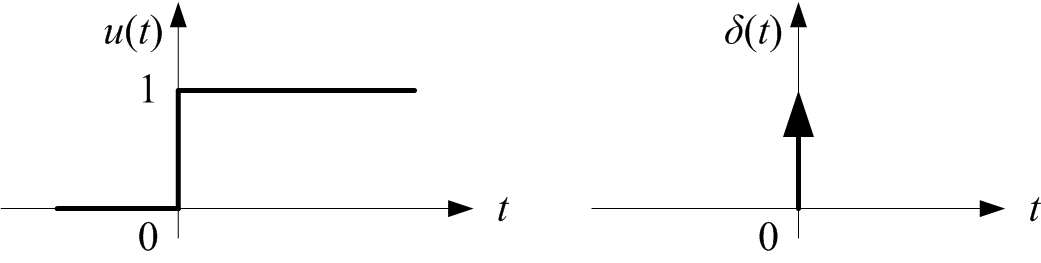
\includegraphics[height=2cm]{1.2.4-1.png}
\end{figure}
\[
u\left( t \right) =\begin{cases}
	1 \quad t\geqslant 0\\
	0 \quad t<0\\
\end{cases} \qquad \begin{array}{l}
	\delta \left( t \right) =0 \quad t\ne 0\\
	\int_{-\infty}^{+\infty}{\delta \left( \tau \right) d\tau}=1\\
\end{array}
\]
两者关系:
\[
\begin{cases}
	u\left( t \right) =\int_{-\infty}^t{\delta \left( \tau \right) d\tau}\\
	\delta \left( t \right) =\frac{du\left( t \right)}{dt}\\
\end{cases}
\]
严格来讲,因为$u\left( t \right) $在$t=0$不连续,所以$\delta \left( t \right) $不是$t=0$的导数。
但不妨碍讨论。

从$u\left( t \right) =\int_{-\infty}^t{\delta \left( \tau \right) d\tau}$来看,$u\left( t \right) $是$\delta \left( t \right) $的积分上限函数,即是积分区间的移动。
令$\tau =t-\sigma $,有:
\begin{align*}
&d\tau =d\left( t-\sigma \right) =-d\sigma \\
&u\left( t \right) =\int_{-\infty}^t{\delta \left( \tau \right) d\tau}=-\int_0^{+\infty}{\delta \left( t-\sigma \right) d\sigma}
\end{align*}
可以认为积分区间不动,$u\left( t \right) $是$\delta \left( t \right) $的移动的结果。
\begin{figure}[h]
\centering
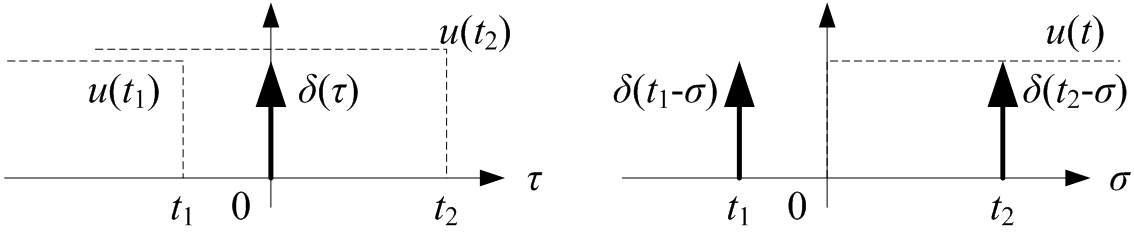
\includegraphics[height=2cm]{1.2.4-2.png}
\end{figure}

$\delta \left( t \right) $的特征:
\begin{itemize}
    \item 偶函数,$\delta \left( t \right) =\delta \left( -t \right) $。
    \item 单位面积,$\int_{-\infty}^{+\infty}{\delta \left( \tau \right) d\tau}=1$,也即能量有限。
    \item 尺度变换性质,$\delta \left( at \right) =\frac{1}{\left| a \right|}\delta \left( t \right) $。
    \item 筛选性,$f\left( t \right) =\int_{-\infty}^{+\infty}{f\left( t \right) \delta \left( \tau -t \right) d\tau}$。
\end{itemize}

$\delta \left( t \right) $的导数:将两个“微小错开”的正负单位冲激的叠加称为{\bf 单位冲激偶},记为$\delta '\left( t \right) $,有如下特征:
\begin{itemize}
    \item 奇函数,$\delta '\left( t \right) =-\delta '\left( -t \right) $。
    \item 面积为0,$\int_{-\infty}^{+\infty}{\delta '\left( \tau \right) d\tau}=0$,也即无能量。
    \item 筛选性,$\int_{-\infty}^{+\infty}{f\left( t \right) \delta '\left( \tau -t \right) d\tau}=-f'\left( t \right) $。
\end{itemize}

%============================================================
\subsection{广义导数}

\begin{definition}[广义导数]
假设信号$x\left( t \right) $在$t_0$不可导,我们定义$x\left( t \right) $在$t_0$的{\bf 广义导数}(generalized derivative)为:
\[
\left. \frac{dx\left( t \right)}{dt} \right|_{t=t_0}=\left[ x\left( {t_0}^+ \right) -x\left( {t_0}^- \right) \right] \delta \left( t-t_0 \right)
\]
即用冲激函数筛选$\left[ x\left( {t_0}^+ \right) -x\left( {t_0}^- \right) \right] \delta \left( t-t_0 \right) $代替$t_0$处的导数。
\end{definition}




